\section{System \"Ubersicht}

\subsection{Komponentendiagramm}

\begin{figure}[H]
  \centering
  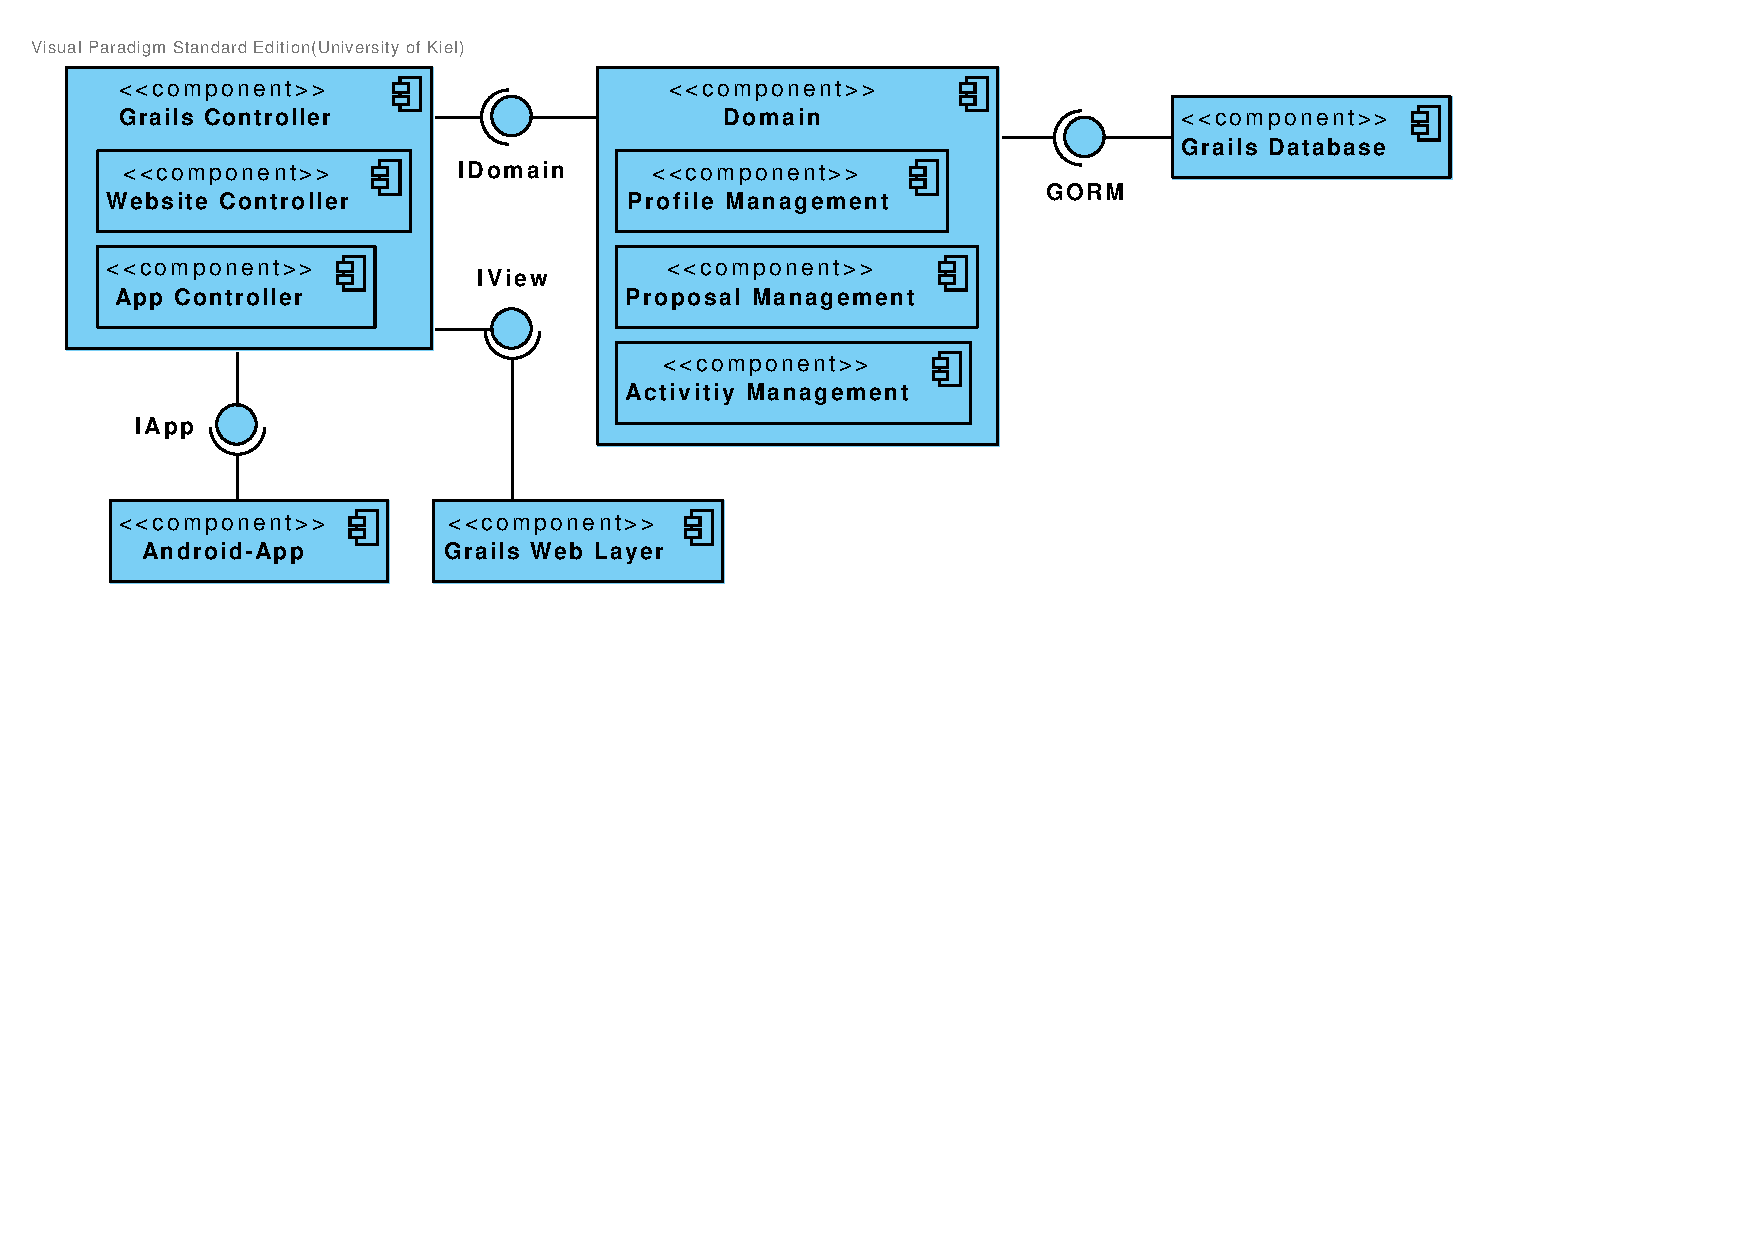
\includegraphics[width=\textwidth, clip]{gfx/component_diagram}
  \caption{Komponentendiagramm}
\end{figure}

\paragraph{Grails Database} Die Grails Database Komponente ist die
zentrale Datenbank, die auf dem Server liegt und s\"amtliche Daten
enth\"alt, auf die \"uber das durch \emph{Grail's Object
  Relational Mapping} (GORM) bereitgestellte Interface zugegriffen werden kann.

\paragraph{Domains} Die Domain Komponente ist die Modell
Repr\"asentation der Daten in der Datenbank. Der Zugriff erfolgt
\"uber das IDomain Interface. Die Domain Komponenten ist unterteilt in
die Subkomponenten \emph{Profile Management}, \emph{Proposal
  Management} und \emph{Activity Management}. Das Profile Management
ist zuständig für die Verwaltung der Modellrepräsentation von Team-
und Benutzerprofilen. Das Proposal Managment ist zuständig für die
Verwaltung der Modellrepräsentation von (Aktivitäts-) Vorschlägen. Die
Komponente Activity Management ist zuständig für die Verwaltung der Modellrepräsentation von Aktivitäten.

\paragraph{Grails Web Layer} Die Grails Web Layer Komponente kommuniziert mit dem Grails Controller \"uber das IView Interface und stellt die GSP Dateien zur Verf\"ugung, die das Layout der Webseite spezifizieren.

\paragraph{Grails Controller} Die Controller Komponente besteht aus den einzelnen Controllern f\"ur Webseite und Android App und ist zust\"andig f\"ur die Verarbeitung s\"amtlicher Daten und Anfragen, die \"uber die IApp, IDomain und IView Schnittstellen kommuniziert werden.

\paragraph{Android App} Die Android App, dient in erster Linie zur Repr\"asentation der Daten vom Server auf Mobilger\"aten. Sie kommuniziert \"uber das IApp Interface mit dem Controller.

\subsection{Verteilungsdiagramm}

\subsubsection{Android-Gerät}
Das Android-Gerät ist das Arbeitswerkzeug für die Benutzer. Auf dem Gerät ist eine native Android-Applikation installiert, mit der Daten eingegeben und abgerufen werden können. Der Benutzer muss bereits registriert sein, um die Applikation nutzen zu können.
\subsubsection{Computer}
Benutzer können mit Hilfe eines Computers über einen Webbrowser auf eine Webseite zugreifen, welche, nach erfolgreichem einloggen, verschiedene Funktionen zur Aktivitäts- und Profilverwaltung anbietet.Des Weiteren können hier auch anonymisierte Statistiken angezeigt und diese statistischen Daten exportiert werden.
\subsubsection{Server}
Der Server stellt die eben erwähnte Webseite bereit. Hier werden gegebenenfalls Datenanfragen von den Android-Geräten verarbeitet.
\subsection{Paketdiagramm}